\documentclass[xcolor=table]{beamer}
\usetheme{metropolis}

\usepackage[utf8]{inputenc}

\usepackage{tikz}
\usetikzlibrary{calc,positioning,arrows,shapes}

\usepackage{subcaption}
\captionsetup{compatibility=false}
\captionsetup{subrefformat=parens}

\usepackage{graphicx}
\usepackage{amsmath}

\usepackage{acronym} % \ac[p], \acl[p], \acs[p], \acf[p]
\usepackage{hyperref}

\usepackage{silence}
\WarningFilter{biblatex}{Patching footnotes failed}
	% Filter warning of biblatex package: "Patching footnotes failed"

\usepackage{appendixnumberbeamer}


% Fixes
% -----

\let\Tiny=\tiny
	% Fix font size wraning.

% References
% ----------


% meta-data
% ---------

\author{Matthieu NICOLAS}
\title{(Ré)Identification efficace dans les types de données répliquées sans conflit (CRDTs)}
%\institute{\includegraphics[scale=0.2]{fig/ul-logo.pdf}\hspace{0.3em}University of Lorraine $|$ \includegraphics[scale=0.08]{fig/inria-logo.pdf}\hspace{0.3em}COAST team $|$ OpenPaaS project\newline \includegraphics[scale=0.2]{fig/supervision-text.pdf}}
\date{Juin 2017}


% Acronyms
% --------

% Presentation
% ------------

\begin{document}
\begin{frame}[t,plain]
\titlepage
\end{frame}

\section{Déroulement de carrière}

%\begin{frame}{Déroulement de carrière}
%  \begin{itemize}
%  \item Études :
%  \end{itemize}
%  \begin{center}
%    \begin{tabular}{cc}
%    \hline
%    \emph{DUT Informatique}   & 2009-2011\\
%    \hline
%    \emph{TELECOM Nancy}      & 2011-2014\\
%    \hline
%    \end{tabular}
%  \end{center}
%
%  \begin{itemize}
%  \item Expériences :
%  \end{itemize}
%  \begin{center}
%    \begin{tabular}{cll}
%    \hline
%    \emph{Ingénieur Jeune Diplômé}    & INRIA, Équipe COAST    & 2014-2016\\
%    \hline
%    \emph{Ingénieur R\&D}             & INRIA, Équipe COAST    & 2016-2017\\
%    \hline
%    \end{tabular}
%  \end{center}
%\end{frame}

\begin{frame}{Déroulement de carrière}
  \begin{itemize}
    \item Études :
    \begin{itemize}
      \item \emph{DUT Informatique}, 2009-2011
      \item \emph{TELECOM Nancy}, 2011-2014
    \end{itemize}
    \item Expériences :
    \begin{itemize}
      \item \emph{Ingénieur Jeune Diplômé}, équipe COAST, 2014-2016
      \item \emph{Ingénieur R\&D}, équipe COAST, 2016-2017
    \end{itemize}
  \end{itemize}
\end{frame}

\section{Projets}

\begin{frame}{Réalisation d'une plateforme d'édition collaborative}
  \begin{itemize}
	\item Contexte
		\begin{itemize}
		\item Équipe COAST a conçu un CRDT, \emph{LogootSplit}
		\item Nécessité d'une preuve de concept
		\end{itemize}
  \item Rôle
		\begin{itemize}
		\item Implémentation de \emph{LogootSplit} sous forme de librairie
		\item Conception et développement de MUTE, un éditeur collaboratif temps réel basé sur cette librairie
		\end{itemize}
  \end{itemize}
\end{frame}

\begin{frame}{Projet OpenPaaS::NG}
  \begin{itemize}
  \item Contexte
		\begin{itemize}
		\item Réalisation d'une suite d'applications collaborative pair-à-pair
		\item En collaboration avec l'équipe DaSciM\footnote{Data Science and Mining} de l'École Polytechnique, Linagora, XWiki SAS et Nexedi
		\item Apporte son expertise sur les mécanismes de réplication de données
		\end{itemize}
  \item Rôle
		\begin{itemize}
		\item Poursuite des travaux sur MUTE
		\item Étude de la littérature sur les CRDTs
		\item Implémentation d'un mécanisme d'anti-entropie
		\item Implémentation d'un mécanisme de livraison des opérations spécifique à \emph{LogootSplit}
		\end{itemize}
	\end{itemize}
\end{frame}

%\section{Sujet}

%\begin{frame}{Sujet}
%  \begin{itemize}
%  \item Porte sur les identifiants des éléments au sein des CRDTs
%  \item Problèmes observés :
%    \begin{itemize}
%    \item Taille non-bornée
%    \item Absence d'un mécanisme de \emph{garbage collection}
%    \end{itemize}
%  \item Pistes de réfléxions :
%    \begin{itemize}
%    \item Mécanisme de garbage collection
%    \item "Remise à plat" de la structure de données
%    \end{itemize}
%  \end{itemize}
%\end{frame}

\section{Motivations}

% TODO: Ajouter une slide sur l'environnement de travail
\begin{frame}{Environnement de travail}
  \begin{itemize}
    \item Laboratoire de recherche
      \begin{itemize}
      \item Animations scientifiques
      \item Diversité des cultures
      \end{itemize}
    \item Équipe COAST
      \begin{itemize}
      \item Sujets de recherches variés
      \item Membres de l'équipe (TODO: Mieux formuler ce point)
      \end{itemize}
    \item Souhaite continuer d'évoluer au sein de cet environnement
  \end{itemize}
\end{frame}

% TODO: Ajouter une slide sur l'enseignement
\begin{frame}{Enseignement}
  \begin{itemize}
  \item Missions d'enseignement
  \item Encadrement de stages et projets
  \item Souhaite m'investir davantage sur cet aspect
  \end{itemize}
\end{frame}

\begin{frame}{Sujet}
  \begin{itemize}
  \item Connaissance des CRDTs
  \item Conscience des avantages de ces structures de données...
  \item ... mais aussi des problèmes existants
  \item Souhaite dorénavant me focaliser sur ces derniers
  \end{itemize}
\end{frame}

\begin{frame}[standout]
  Merci pour votre attention, avez-vous des questions ?
\end{frame}

%%%%%%%%%%%%%%%%%%%%%%%%%%%%%%%%%%%%%%%%%%%%%%%%%%%%%%%%%%%%%%%%%%%%%%%%%%%%%%%
\appendix

\begin{frame}{MUTE}
  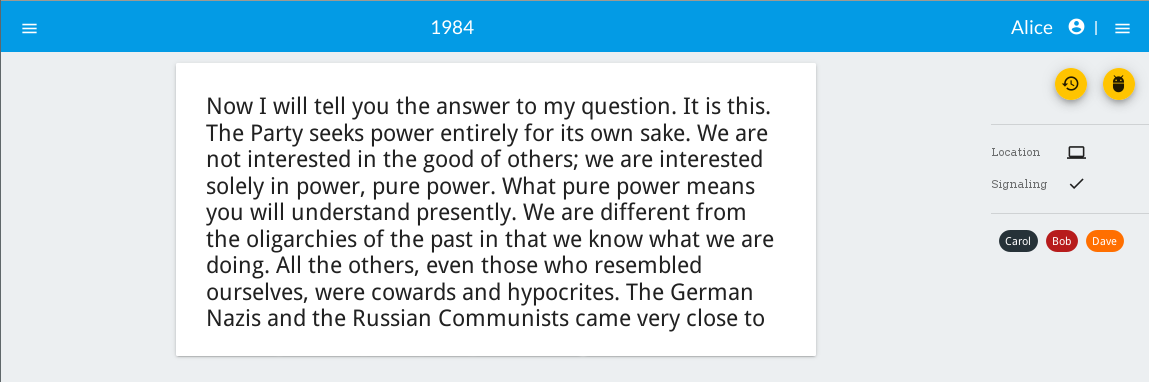
\includegraphics[scale=0.28]{fig/MUTE.png}
\end{frame}

\end{document}
